\chapter{Research methodology and implementation}
In this chapter the author is designing the methodology to be followed in the experiments. This is an important step, as building it correctly will lead to significant and meaningful results.
We discuss three phases: data acquisition and preprocessing, price forecasting and predictor's importance.

In the first phase, all the necessary data will be downloaded with the finest possible granularity.
When studying broader timespans, it will be aggregated.

In the last two phases the author explains the design of the experiments: the same procedure will be used to analyze in an hourly, daily and monthly fashion, changing the parameters for every case.
On the other hand, for the yearly level, as there is not enough data to perform an statistical study, a descriptive and visual analysis will be performed.

\section{Data acquisition and preprocessing}

\section{ML models need tabular form}
In statistical time series models as ARIMA, data can be directly introduced in the model without restructuring it.
But when we use ML-based architectures, data has to be reshaped so the models can recover autocorrelation.
This is why the author arranges it in the tabular form described in Figure \ref{fig:ml-arrangement}.
On it, the response (price) and predictors (as could be demand or generation) are included together with some response lags.

\begin{figure}[H]
\centering
    \caption{Tabular form in which data is disposed for ML models. On it, n is the number of observations in the time series and k is the number of lags in use.}
    \label{fig:ml-arrangement}
    \fbox{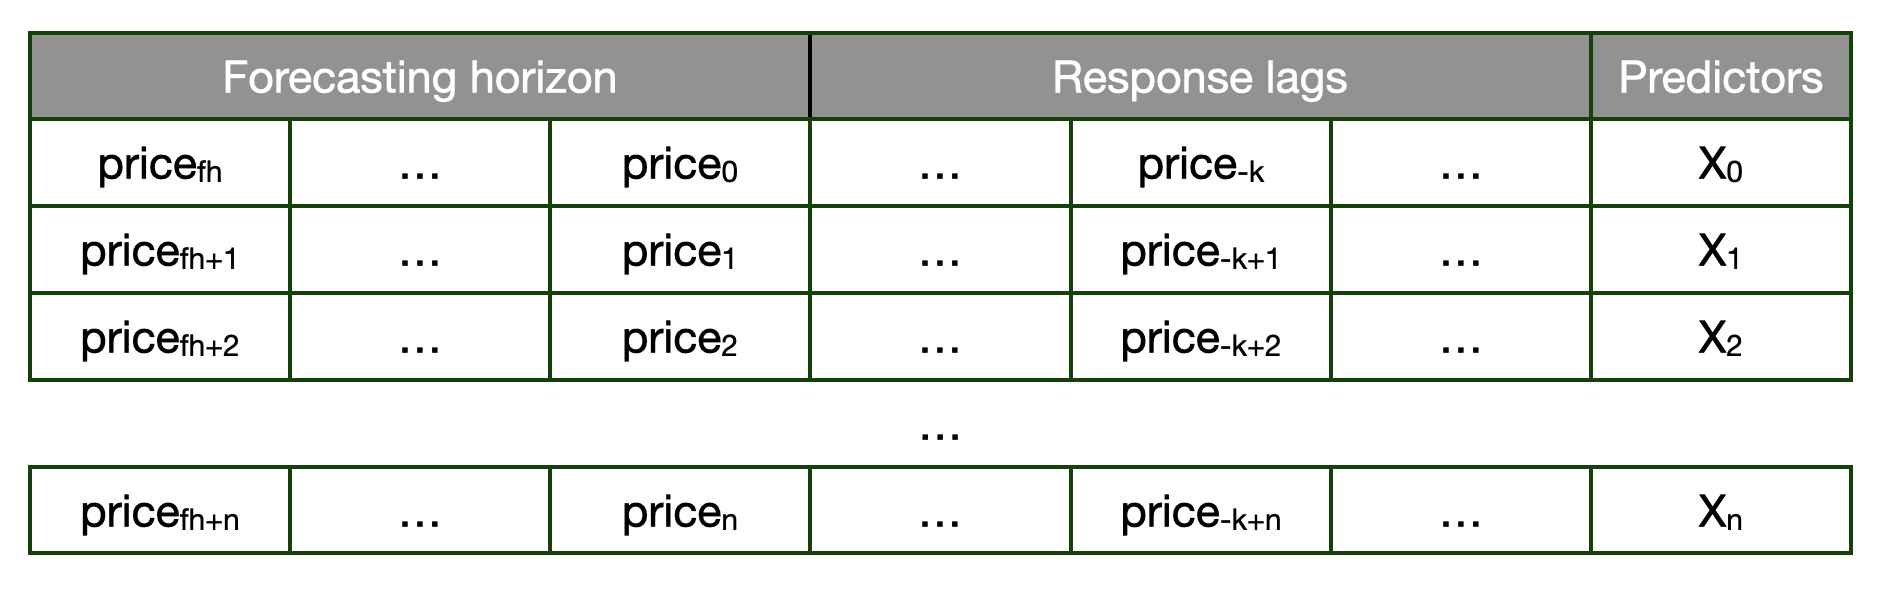
\includegraphics[scale=0.4]{images/methodology/ml_arrangement}}
\end{figure}

The author has decided to implement this table generation manually, to exactly control the lags to use on each case.

\section{Price forecasting}
The library used to perform forecasts is \textit{sktime}: it simplifies the implementation, reducing boilerplate code and making the scripts cleaner.

\subsection{Models to compare}
We will test different models, analyzing which of them work better:
\begin{itemize}
    \item k-Nearest Neighbors (kNN)
    \item Random Forest (RF)
    \item Gradient Boosted Trees (GBT)
    \item Support Vector Machine (SVM)
    \item Dummy regressor, acting as baseline.
\end{itemize}
All of them are implemented in \textit{scikit-learn} and integrated in \textit{sktime} by the use of \textit{make\_reduction()} function. On it, the parameter \text{strategy} needs to be specified: there are two possible strategies to forecast each value in the forecasting horizon, direct and recursive.

The former creates one model for each value in the forecasting horizon, the latter applies a recursive process in which each new prediction is based on the previous one \cite{direct-recursive-forecasting}, so only one model is created. See Figure \ref{fig:direct-recursive-forecasting}. Direct strategy is what is used on this project, as it is more precise. On the other hand, it is computationally expensive.

\begin{figure}[H]
\centering
    \begin{subfigure}{.45\textwidth}
        \centering
        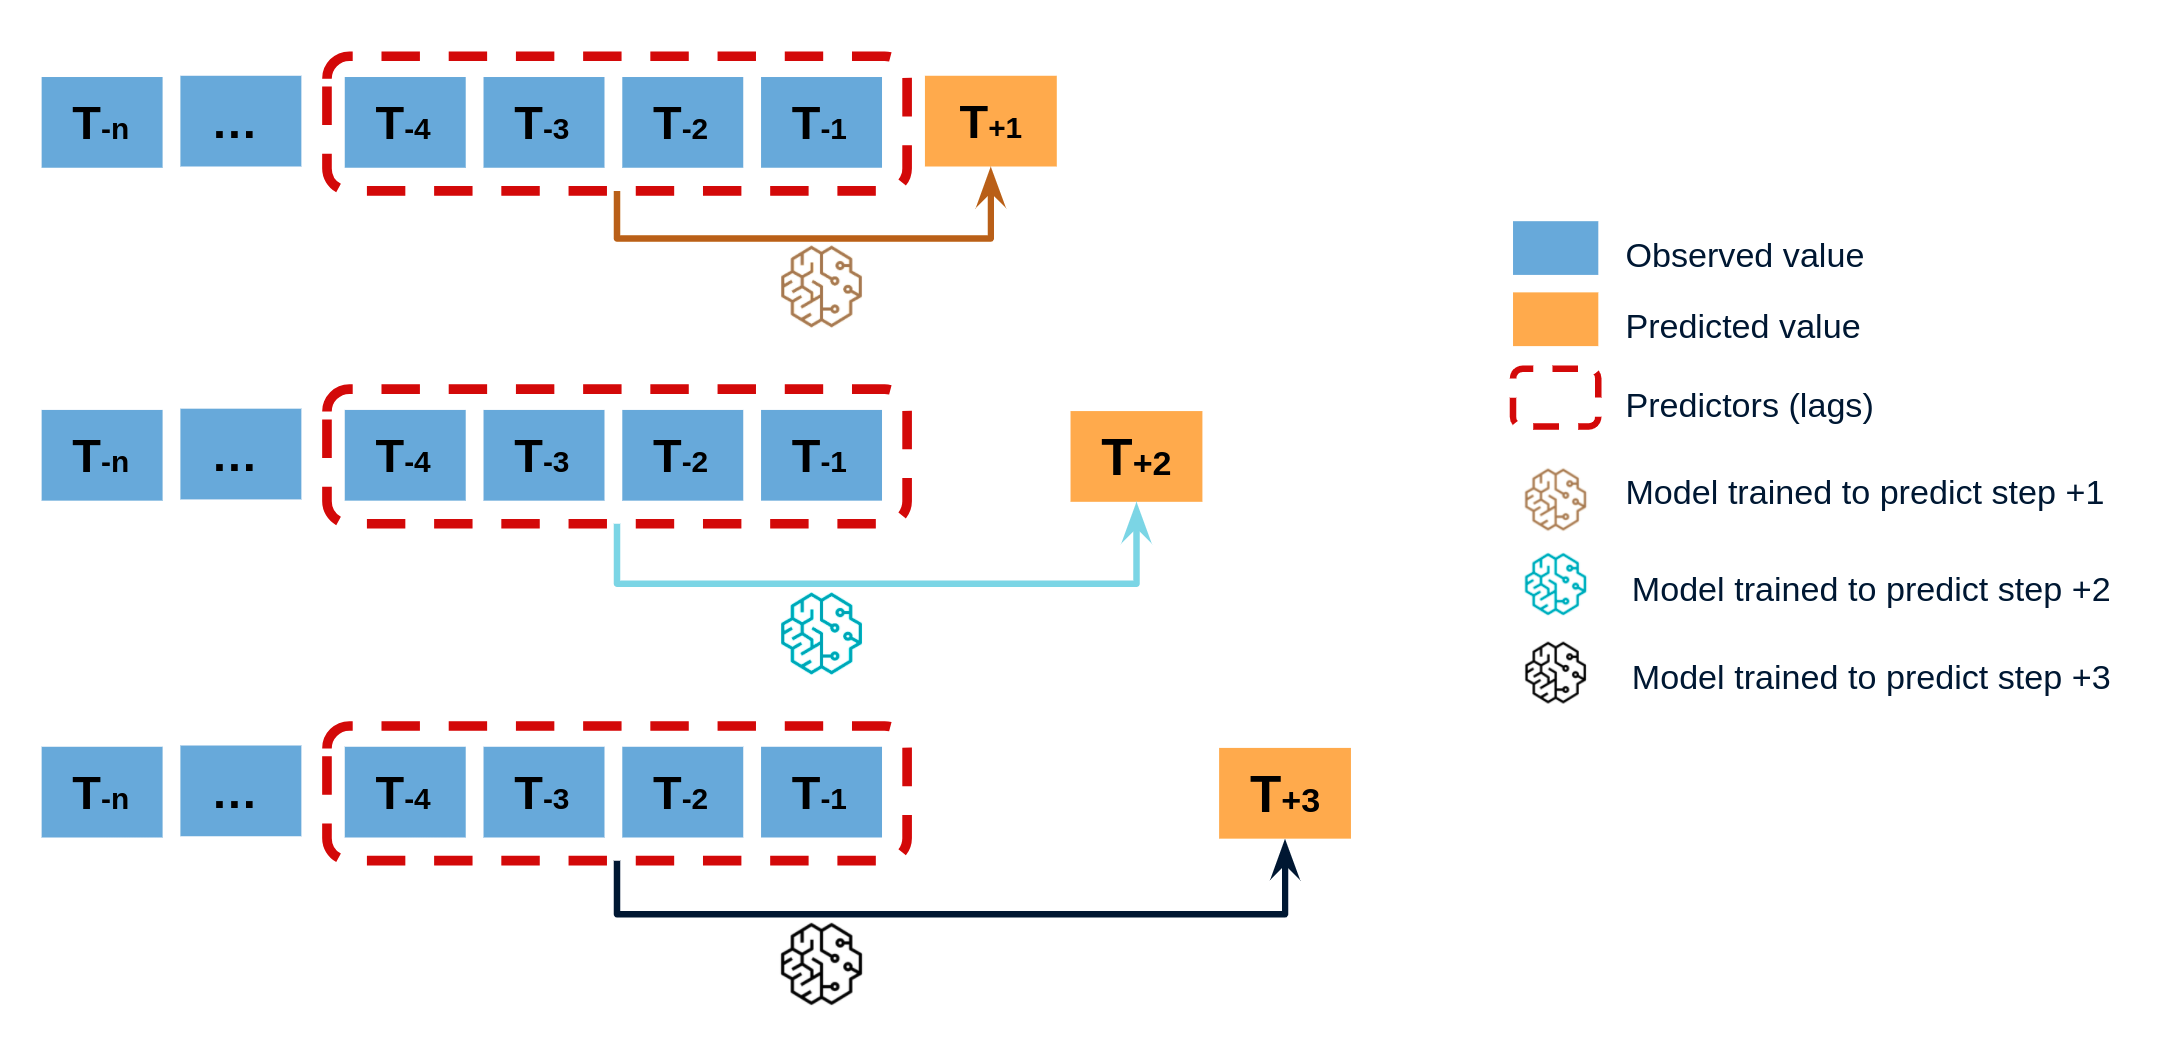
\includegraphics[width=1\linewidth]{images/methodology/direct-multi-step-forecasting}
        \caption{Direct forecasting.}
    \end{subfigure}
    \begin{subfigure}{.45\textwidth}
        \centering
        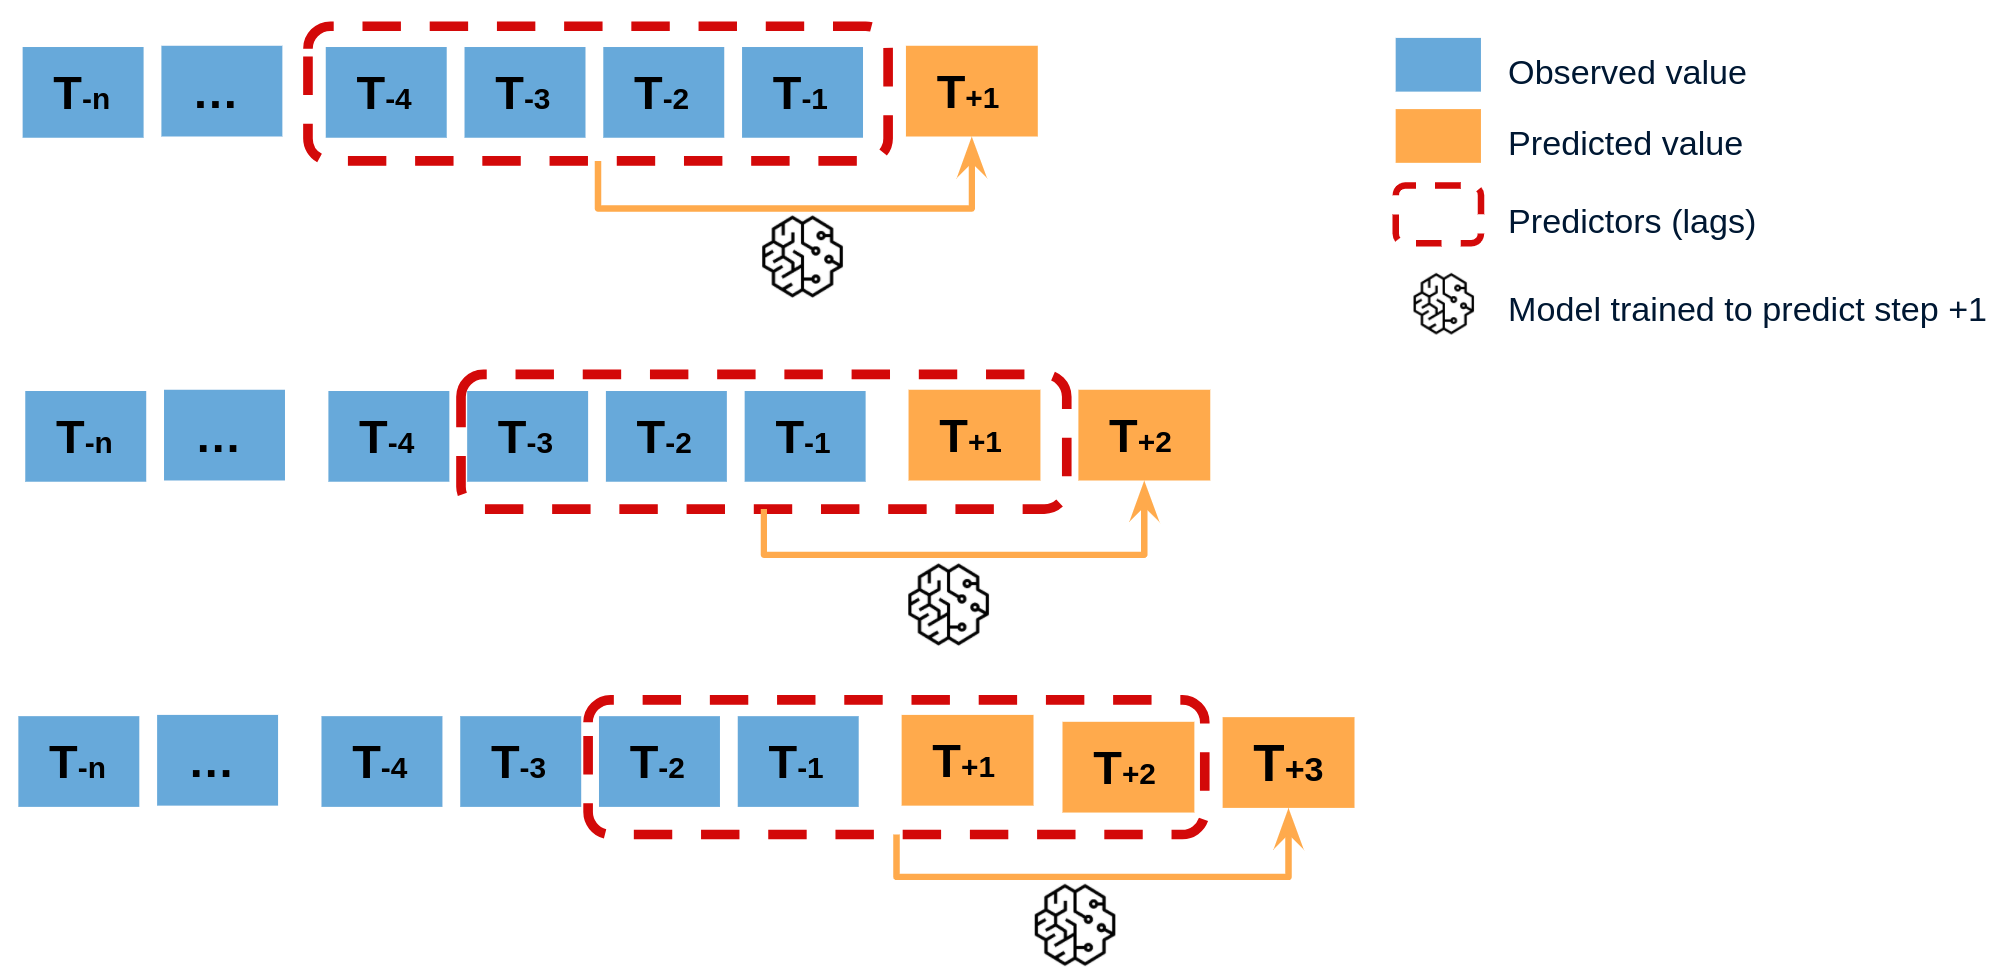
\includegraphics[width=1\linewidth]{images/methodology/recursive-mutistep-forecasting}
        \caption{Recursive forecasting.}
    \end{subfigure}

    \caption{Direct vs recursive forecasting strategies.}
    \label{fig:direct-recursive-forecasting}
\end{figure}

To compare the performance between different models, the author will use the Mean Scaled Absolute Error (MASE) loss function described in Equation \ref{eq:mase}:
\begin{equation}
    \label{eq:mase}
    \mathrm{MASE} = \frac{1}{N}\sum_{k=1}^{N}\frac{|p_k-\hat{p}_k|}{\frac{1}{n-1}\sum_{i=2}^{n} |p^\mathrm{in}_i - p^\mathrm{in}_{i-1} |},
\end{equation}

\subsection{Performance evaluation}
This process will be performed in two steps. In the first, we compare the performance of the different models using cross validation. Once we know which returns the higher score, we train it over all the cross-validation data and give a final estimation over a test set. See Figure \ref{fig:cross-train-test}.

\begin{figure}[H]
\centering
    \caption{Data splitting to peform model selection and final model performance estimation.}
    \label{fig:cross-train-test}
    \fbox{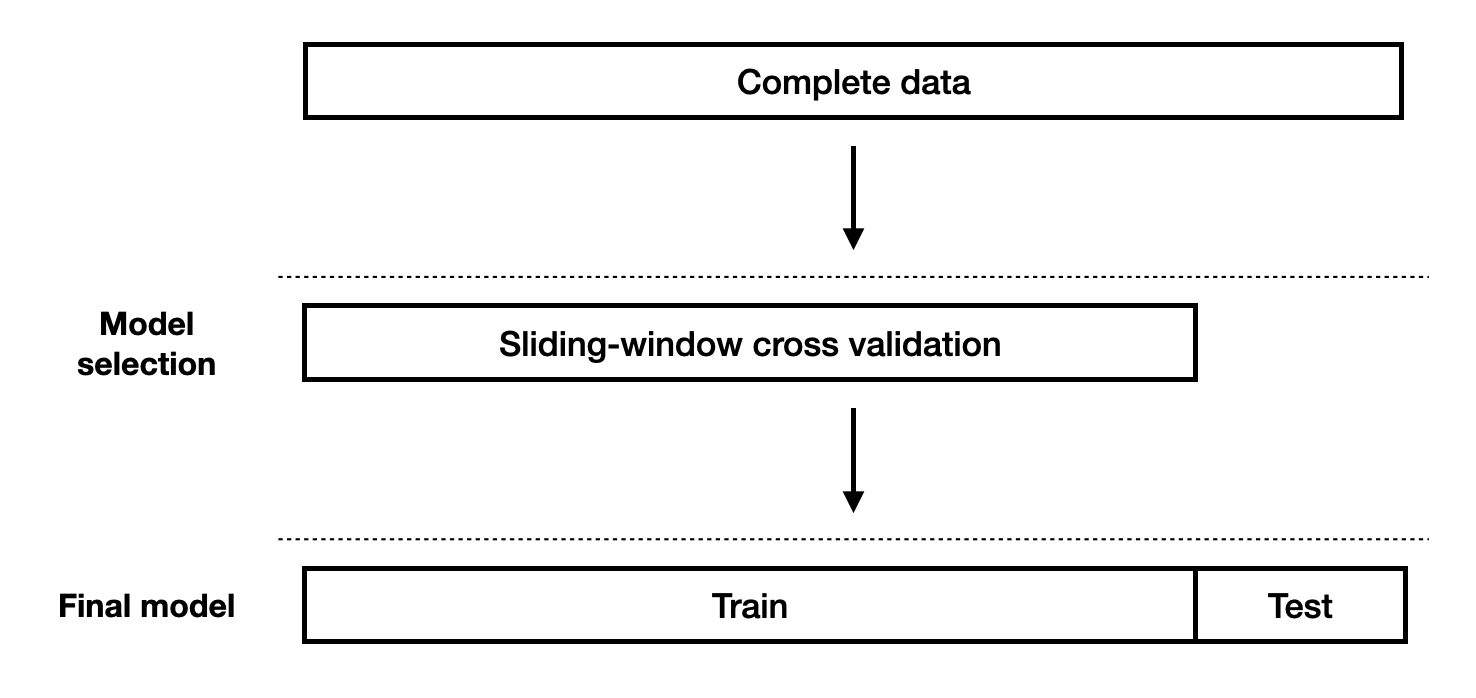
\includegraphics[scale=0.4]{images/methodology/cross_train_test}}
\end{figure}

\subsubsection{Model selection}
Two well known strategies used to divide data to perform model selection are holdout and cross-validation.
In the former, data is partitioned in two splits, train and test, e.g. 80\% train and 20\% test.
The problem with this strategy is that we are only assessing the performance of the model in a reduced portion of data.
On the other hand, if we use cross-validation we divide the data in multiple folds: on an iterative process, one is reserved for testing and the rest for training, changing the test fold on every iteration.
At the end, we manage to assess the performance in the complete dataset.

\noindent But using k-fold cross validation is not suitable for time series forecasting \cite{cross-validation-types}:
\begin{enumerate}
    \item Test data can appear before train data.
    \item Data leakage can happen if test data appears after train folds, as the model knows extra information about the future.
\end{enumerate}

There exist other techniques that solve this problem, for example sliding or expanding window cross validation.
In sliding window splitters, the folds are created by scrolling a window of constant size through data.
This window is divided into train and test, maintaining the size of both partitions on all the windows.

In the case of expanding windows, its size is not constant but it grows. Concretely, the test partition remains the same through different windows and the train one grows collecting all the previous observations.

In Figure \ref{fig:sliding-expanding-windows} the author exposes a comparison between both strategies. For this project we are using sliding windows.

\begin{figure}[H]
\centering
    \caption{Sliding vs expanding windows \cite{sliding-expanding-windows}.}
    \label{fig:sliding-expanding-windows}
    \fbox{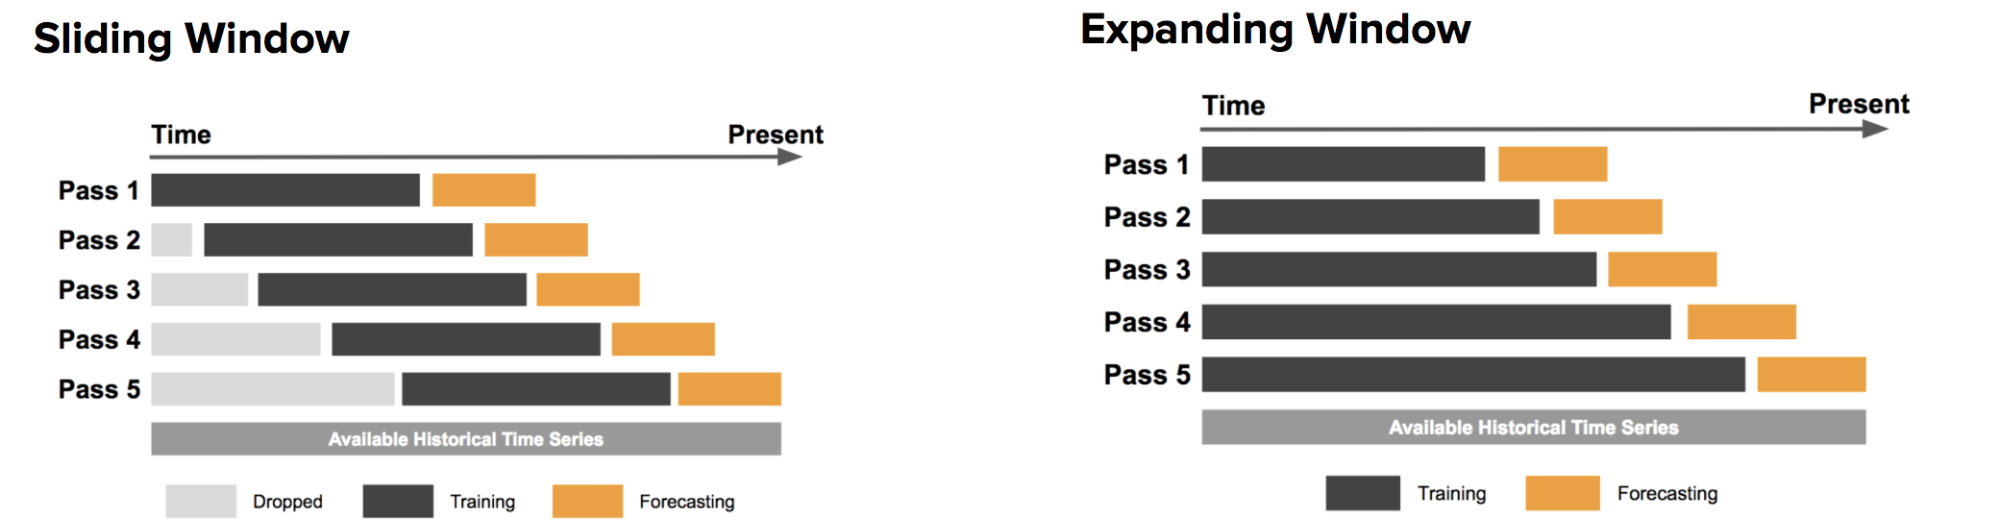
\includegraphics[scale=0.2]{images/methodology/sliding-expanding-windows}}
\end{figure}

Once that the data has been preprocessed and the cross-validation pipeline has been built, is time to run it.
The results will indicate which is the most suitable model on each case.

\subsubsection{Best model forecast}
Now that the most suitable model is known, it is trained over the data used for cross validation and tested  over new data that haven't been used previously.
That data corresponds to the newest values in the series.

This will be the final prediction shown in this report, together with a final performance estimation.

\section{Predictor's importance with SHAP values}
As we studied in Chapter \ref{ch:state-of-the-art}, SHAP values are a state-of-the-art way of explaining predictor's importance in ML models. Unluckily, the existing implementations are not compatible with \textit{sktime}. On the other hand, the implementation in \cite{shap-package} works with \textit{scikit-learn} models.

To study which variables affect the electricity price, a different strategy to what is done in forecasting is followed. Instead of training a model for each point in the forecasting horizon, we only create for the first and last values. Over the results of this two models we will apply the SHAP computation.

The study is performed in this way because interpreting SHAP values for each individual forecast horizon point is not viable. Another option would be to average the SHAP values for all the points, but the author thinks that this will make the results less interpretable.

The architecture used for the two models is the one that returned the best result in forecasting. They work over tabular data disposed like in Figure \ref{fig:shap-arrangement}. Once tabulated, data is divided into train and test (Figure \ref{fig:shap-train-test}): the train split is used to train the models and the test partition is the one over the SHAP value are computed.

\begin{figure}[H]
\centering
    \begin{subfigure}{.95\textwidth}
        \centering
        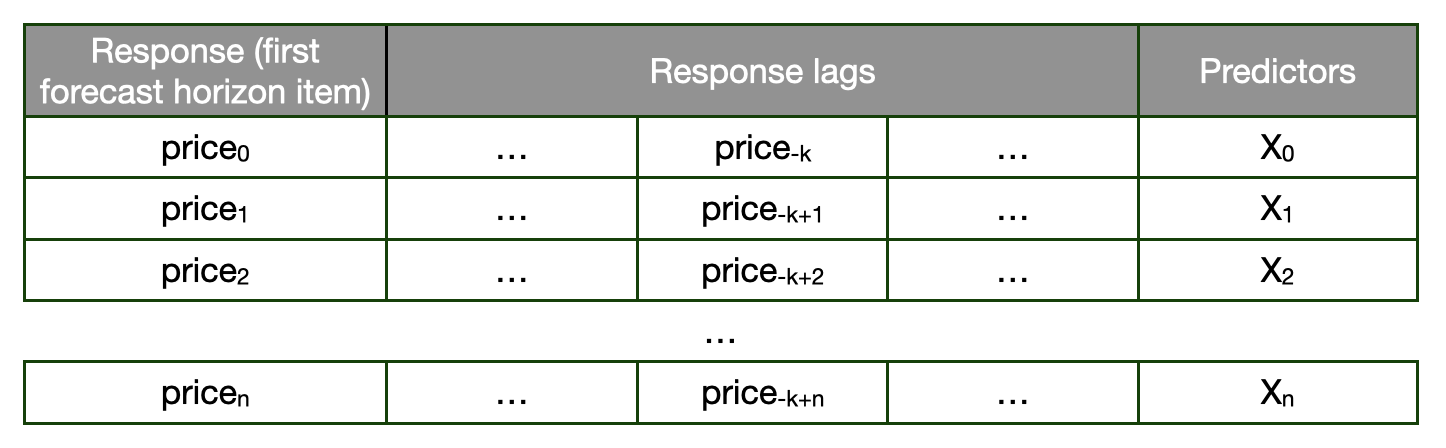
\includegraphics[width=1\linewidth]{images/methodology/shap_arrangement_first}
        \caption{Disposition for the first value case in the forecasting horizon.}
        \label{fig:shap-arrangement-first}
    \end{subfigure}
    \vspace{0.3cm}
    \begin{subfigure}{.95\textwidth}
        \centering
        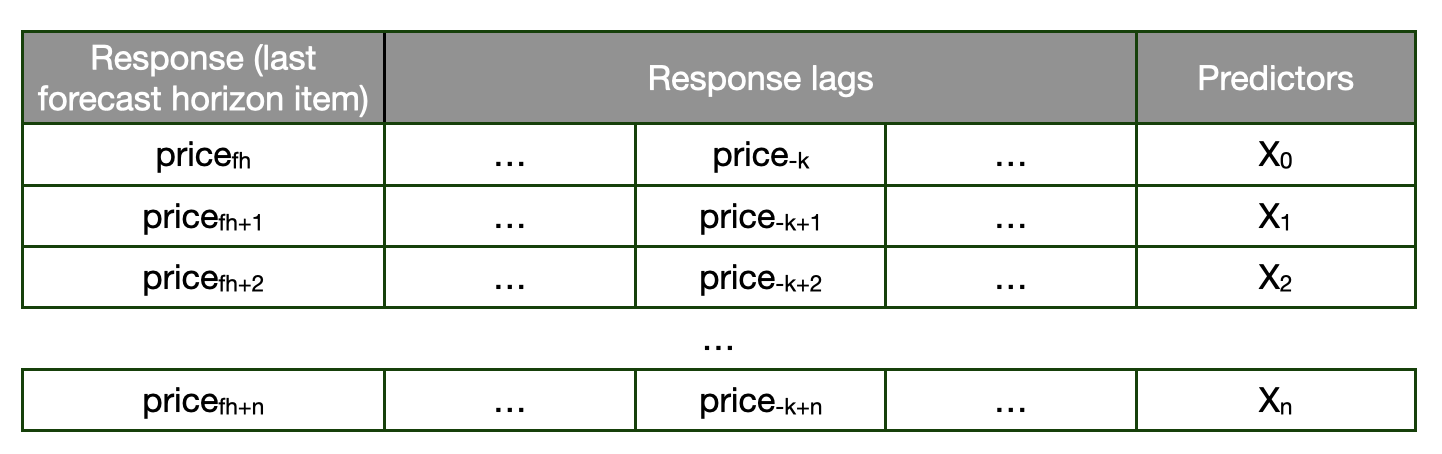
\includegraphics[width=1\linewidth]{images/methodology/shap_arrangement_last}
        \caption{Disposition for the last value case in the forecasting horizon.}
        \label{fig:shap-arrangement-last}
    \end{subfigure}

    \caption{Data disposition to evaluate the influence of predictors.}
    \label{fig:shap-arrangement}
\end{figure}

\begin{figure}[H]
\centering
    \caption{Train/test split of the tabular data used to compute the SHAP values.}
    \label{fig:shap-train-test}
    \fbox{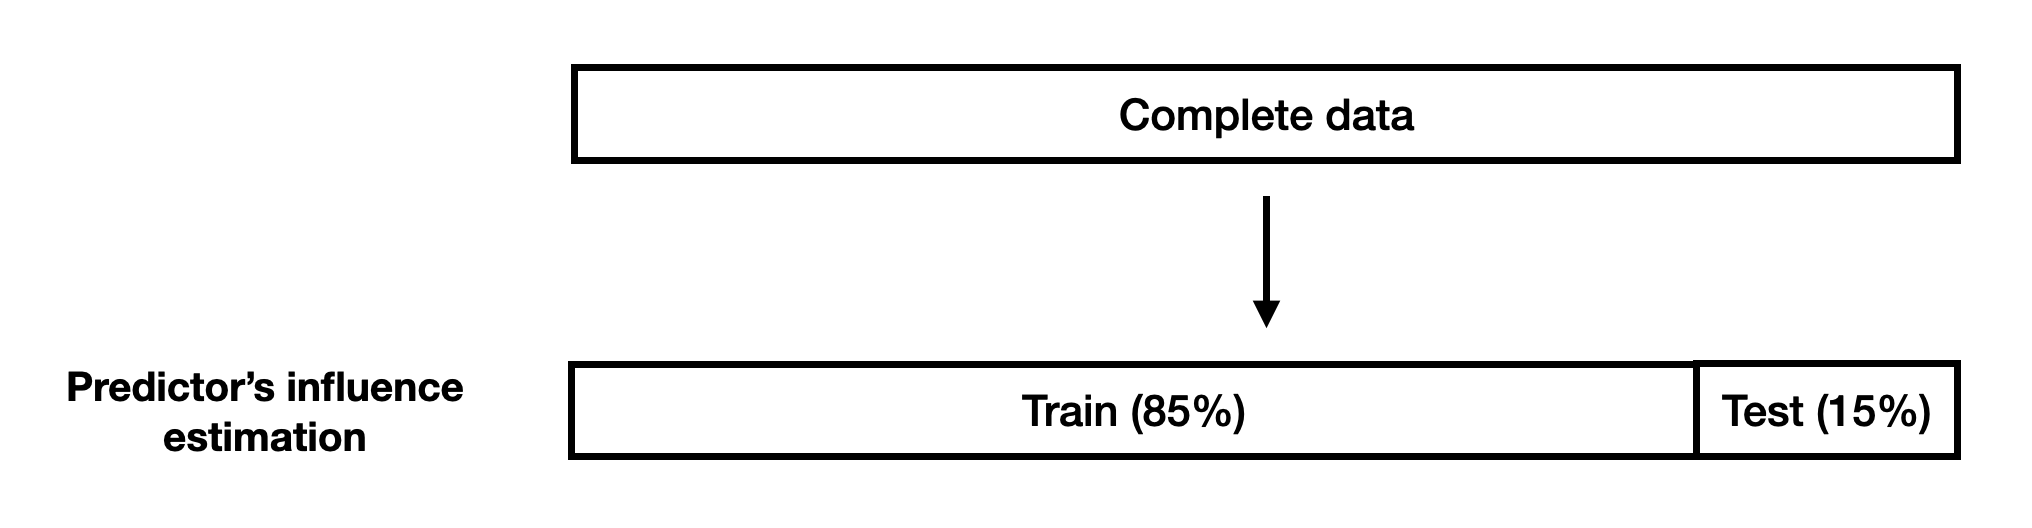
\includegraphics[scale=0.38]{images/methodology/shap_train_test}}
\end{figure}


%\section{Yearly forecasting}
%Judgmental forecasting